% Figure for scale_lanes_deck: two ways to use a session — fresh per episode, or kept per lane.
% Build: xelatex lanes_fig04_session-use.tex  (-> .pdf, included by ../scale_lanes_deck.md)
\documentclass[tikz,border=4pt]{standalone}
\usepackage{fontspec}
\setmainfont{DejaVu Sans}
\setmonofont{DejaVu Sans Mono}
\usetikzlibrary{arrows.meta}
\definecolor{slime}{RGB}{230,230,230}
\definecolor{vm}{RGB}{214,238,220}
\definecolor{bad}{RGB}{245,205,205}
\definecolor{ink}{RGB}{40,40,90}
\begin{document}
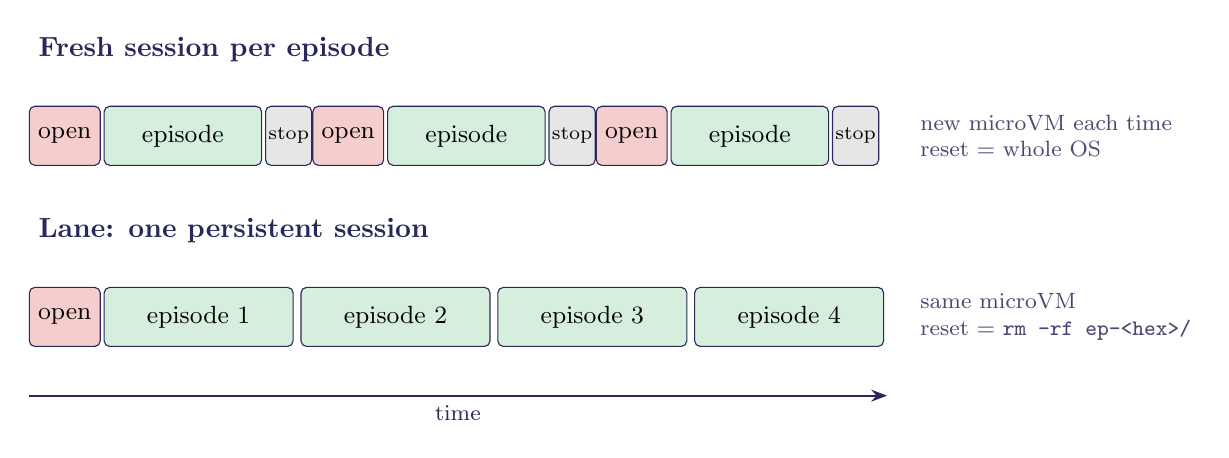
\begin{tikzpicture}[
  font=\small,
  blk/.style={draw=ink, rounded corners=2pt, fill=#1, minimum height=0.75cm, inner sep=1pt, anchor=west},
  head/.style={font=\bfseries, text=ink, anchor=west},
  note/.style={font=\footnotesize, text=ink!85, anchor=west, align=left},
]
% Row A: fresh per episode — open | episode | stop, three times
\node[head] at (0,1.1) {Fresh session per episode};
\foreach \k in {0,1,2} {
  \pgfmathsetmacro{\x}{\k*3.6}
  \node[blk=bad, minimum width=0.9cm] at (\x,0) {open};
  \node[blk=vm, minimum width=2.0cm] at (\x+0.95,0) {episode};
  \node[blk=slime, minimum width=0.55cm] at (\x+3.0,0) {\scriptsize stop};
}
\node[note] at (11.2,0) {new microVM each time\\reset = whole OS};
% Row B: lane — open once, then episodes back to back
\node[head] at (0,-1.2) {Lane: one persistent session};
\node[blk=bad, minimum width=0.9cm] at (0,-2.3) {open};
\foreach \k in {0,1,2,3} {
  \pgfmathsetmacro{\x}{0.95+\k*2.5}
  \node[blk=vm, minimum width=2.4cm] at (\x,-2.3) {episode \pgfmathparse{int(\k+1)}\pgfmathresult};
}
\node[note] at (11.2,-2.3) {same microVM\\reset = \texttt{rm -rf ep-<hex>/}};
\draw[thick, ink, -{Stealth[length=2mm]}] (0,-3.3) -- (10.9,-3.3) node[midway, below, font=\footnotesize, text=ink] {time};
\end{tikzpicture}
\end{document}
